\documentclass[a4paper,12pt]{article}
\usepackage[utf8]{inputenc}
\usepackage{geometry}
\usepackage{longtable}
\usepackage{booktabs}
\usepackage{enumitem}
\usepackage{xcolor}
\usepackage{caption}
\usepackage{graphicx}
\usepackage{float}

\geometry{margin=1in}

\title{\textbf{Personal Investment Report for 2025 Q2}}
\author{Yi-Fan Chen}
\date{June 30, 2025}

\begin{document}

\begin{titlepage}
    \centering
    \vspace*{\fill}
    {\Huge \textbf{PIGU INVESTMENT, INC.} \par}
    \vspace{1.5cm}
    {\LARGE Balance Sheet \par}
    \vspace{2cm}
    {\Large June 2025 Quarter 2 \par}
    \vspace*{\fill}
\end{titlepage}


\section{Introduction}
This report provides an overview of my investment portfolio as of June 2025, including current holdings, realized and unrealized gains/losses, and cash reserves.

\section{Current Holdings (NTD)}
\begin{longtable}{llllll}
    \toprule
    Stock Code & Shares & Avg. Purchase Price & Current Market Price & Cost & Value \\
    \midrule
    2916 Munsin       & 750  & 46.35 & 46.25 & 34,762.5 & 34,687 \\
    2912 President Chain & 150 & 254.0  & 256.5  & 38,100  & 38,475 \\
    2379 Realtek      & 70   & 480.64 & 567.0 & 33,644.8 & 39,690 \\
    2610 China Air    & 500  & 19.3   & 21.6  & 9,650   & 10,800 \\
    2330 TSMC         & 110  & 800.0 & 1,060.0 & 88,000  & 116,600 \\
    \bottomrule
\end{longtable}
\textbf{Total Unrealized Gain:} \textcolor{blue}{36,094.7} NTD

\section{Realized Gains/Losses (NTD)}
\begin{longtable}{lllll}
    \toprule
    Stock Code & Shares & Buy Price & Sell Price & Gain/Loss \\
    \midrule
    2882 Cathay Financial & 1,000 & 62.589 & 69.4 & 6,505 \\
    2882 Cathay Financial & 1,000 & 55.679 & 66.6 & 10,628 \\
    4938 Pegatron & 100 & 73.0 & 86.0 & 1,252 \\
    2382 Quanta & 50 & 190.76 & 253.0 & 3,057 \\
    2884 E.SUN Financial & 1,020 & 22.61 & 29.05 & 6,409 \\
    2379 Realtek & 100 & 440.0 & 512.0 & 7,120 \\
    \bottomrule
\end{longtable}

\textbf{Total Realized Loss:} \textcolor{blue}{34,971} NTD

\section{Stock Equity Distribution}
\begin{figure}[H]
    \centering
    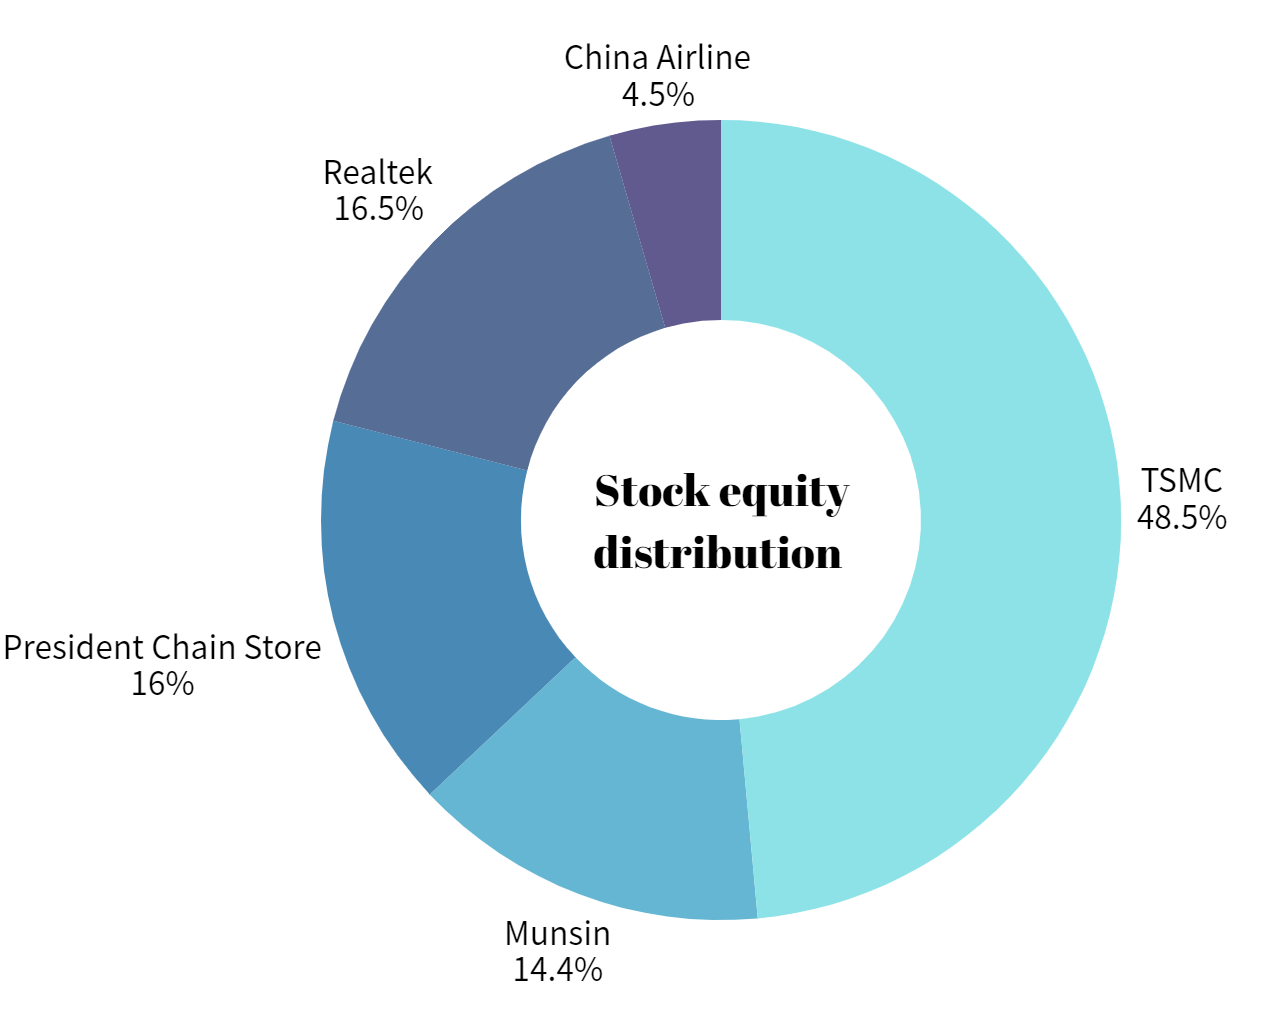
\includegraphics[width=0.8\textwidth]{stock_equity_distribution.png}
    \caption{Stock Equity Distribution as of 2025 Q2}
    \label{fig:stock_equity_distribution}
\end{figure}

\noindent The figure below illustrates the distribution of stock equity in my portfolio as of the second quarter of 2025. It provides a visual representation of the proportion of each stock's value relative to the total portfolio value.


\section{Cash \& Fixed Deposits}
\begin{longtable}{ll}
    \toprule
    Type & Amount (NTD) \\
    \midrule
    USD Fixed Deposit (9,628 USD @ 29.0) & 279,212 \\
    TWD Cash                             & 220,000 \\
    JPY           (100,000 JPY @ 0.2091) & 20,910 \\
    \bottomrule
    \textbf{Total Cash} & 520,122 \\
\end{longtable}

\textbf{Foreign Exchange Loss (compare to the 1st quarter):} \textcolor{red}{-37,549.2} NTD

\noindent
\section{Total Equity}
\begin{longtable}{ll}
    \toprule
    \multicolumn{2}{l}{\textbf{Liabilities}} \\
    \midrule
    \textbf{Current Liabilities} & \\
    Short Term Debt & 80,000.00 \\
    \textbf{Non Current Liabilities} & \\
    Long Term Debt & 0.00 \\
    \midrule
    \textbf{Total Liabilities} & \underline{80,000.00} \\
    \\
    \multicolumn{2}{l}{\textbf{Equity}} \\
    \midrule
    Total Portfolio Value (Holdings) & 240,252.00 \\
    Total Cash \& Fixed Deposits      & 520,122.00 \\
    \midrule
    \textbf{Total Equity} & \underline{760,374.00} \\
    \\
    \textbf{Net Worth (Equity - Liabilities)} & \textbf{680,374.00} \\
    \bottomrule
\end{longtable}


\end{document}
